% pyFormex manual (we use the python manual class)
%
\documentclass[a4paper]{manual}
%
%% Dirty hack to make Python classes work together with hyperref
\let\pyurl\url
\let\url\relax
%%
\usepackage{hyperref}
%\usepackage[latex2html]{hyperref}
%\usepackage[latex2html,pdftex]{hyperref}
\usepackage{html}
\usepackage{xspace}
\usepackage{graphicx}
\usepackage{subfigure}
%\usepackage[pdftex]{graphicx}
\title{pyFormex manual}
\author{Tim Neels and Benedict Verhegghe}
\release{0.3-alpha}
\setshortversion{0.3}
\newcommand{\pyformex}{pyFormex\xspace}
\newcommand{\websiteURL}{http://pyformex.berlios.de\xspace}
%\newenvironment{mycode}{\par\small\sffamily}{} % This should be changed
 

\begin{document}
\maketitle
\chapter{Introduction}
\label{cha:introduction}

\section{What is \pyformex{}?}
\label{sec:what-pyformex}
You probably expect to find here a short definition of what \pyformex is and what it can do for you. I may have to disappoint you: describing the essence of \pyformex in a few lines is not an easy task to do, because the program can be (and is being) used for very different tasks. So I will give you two answers here: a short one and a long one.

The short answer is that \pyformex{} is a program to \emph{generate large structured sets of coordinates by means of subsequent mathematical transformations gathered in a script.}
If you find this definition too dull, incomprehensible or just not descriptive enough, read on through this section and look at some of the examples in this manual and on the \htmladdnormallinkfoot{\pyformex website}{\websiteURL}. You will then probably have a better idea of what \pyformex{} is. 

The initial intention of \pyformex{} (and probably still its main use) was the rapid design of three-dimensional wireframe structures with a configuration that can easier be obtained through mathematical description than through interactive generation of its subparts and assemblage thereof.

The example of the stent\footnote{A stent is a tube-shaped structure that is e.g. used to reopen (and keep open) obstructed blood vessels.} in the figure below illustrates this clearly. 

\begin{figure}[h]
  \begin{makeimage}
  \end{makeimage}
  \centering
  %\htmlimage{scale=0.5}
  \begin{latexonly}
  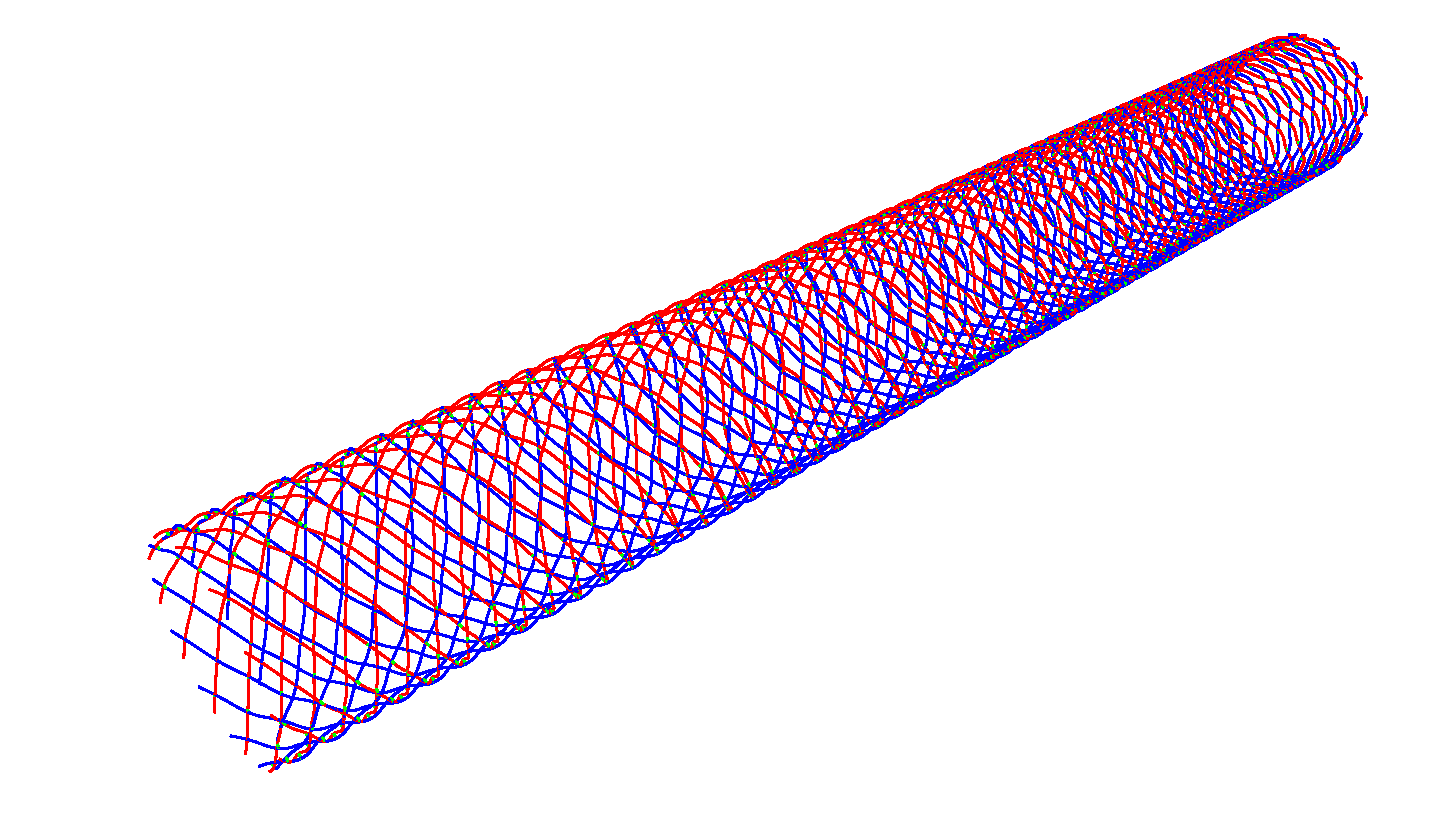
\includegraphics[width=12cm]{images/wirestent}
  \end{latexonly}
  \begin{htmlonly}
    %\hyperimage{../../examples/wirestent.png}
    \htmladdimg{../images/wirestent.png}
  \end{htmlonly}  \caption{WireStent example.}
\end{figure}


The structure has ...


\section{History}
\label{sec:history}

\section{Quick tutorial for the \pyformex{} GUI}
\label{sec:gui-tutorial}
In the current version () the GUI mainly serves the following purposes:
\begin{itemize}
\item Display a structure in 3D. This includes changing the viewpoint, orientyation and viewing distance. Thus you can interactively rotate, translate, zoom.
\item Save a view in one of the supported image formats. Most of the images in this manual and on the \pyformex{} website were created that way. 
\item Changing \pyformex settings (though there aren't many yet that can be changed through the GUI).
\item Running \pyformex scripts, possibly starting other programs and display their results.
\end{itemize}

The GUI does not (yet) provide a means to interactively design a structure, select parts of a structure or set/show information about (parts of) the structure. Designing a structure is done by writing a small script with the mathematical expressions needed to generate it. Any text editor will be suitable for this purpose. The author uses XEmacs, but this is just a personal preference. 
A Python aware editor is preferable though, because that is the language used in pyFormex scripts.
A \pyformex editor integrated into the GUI remains on our TODO list, but it certainly has not our top priority, because general purpose editors are adequate for most of our purposes. 

The best way to learn to use pyFormex is by studying and changing some of the examples. I suggest that you first take a look at the examples included in the pyFormex GUI and select those that display structures that look interesting to you. Then you can study the source code of those examples and see how the structures got built. 
When starting up, \pyformex reads through the Examples directory (this is normally the 'examples' subdirecty located under the pyformex installation dir).  
\menuselection{Examples \sub WireStent}


\section{Quick NumPy tutorial}
\label{sec:numpy-tutorial}
This could be part of the tutorial in chapter 2

%%%%%%%%%%%%%%%%%%%%%%%%%%%%%%%%%%%%%%%%%%%%%%%%%%%%%%%%%%%%%%%%%%%%%%%%%%%
\chapter{pyFormex --- a tutorial}
{\label{cha:tutorial}

\section{Introduction}

PyFormex is a Python implementation of Formex algebra. Using pyFormex, it is very easy to  generate large geometrical models of 3D structures by a sequence of mathematical transformations. It is especially suited for the automated design of spatial frame structures. But it can also be used for other tasks, like finite element preprocessing, or just for creating some nice pictures.

By writing a very simple script, a large geometry can be created by copying, translating, rotating,... Formices.  

\section{General remarks}

The model will be generated by pyFormex, based on a script. PyFormex will interpret this script and draw what you have created. This is clearly very different than the traditional way of creating a model, like CAD. There are two huge advantages about using pyFormex

\begin{itemize}
\item It is especially suited for the automated design of spatial frame structures. A dome, arc, hypar,... can be rather difficult to draw with CAD, but when using mathematical transformations, it becomes a piece of cake!
\item Using a script makes it very easy to apply changes in the geometry: you simply modify the script and let pyFormex play it again. For instance, you can easily change an angle, the radius of a dome, the ratio f/l of an arc,... Using CAD, you would have to make an entirely new drawing! This is also illustrated in fig \ref{scallops}: these domes where all created with the same script, but with other values of the parameters.
\end{itemize}

\begin{figure}[tbp,h]
\centering
  \subfigure[A basic Scallopdome]{\label{scallop}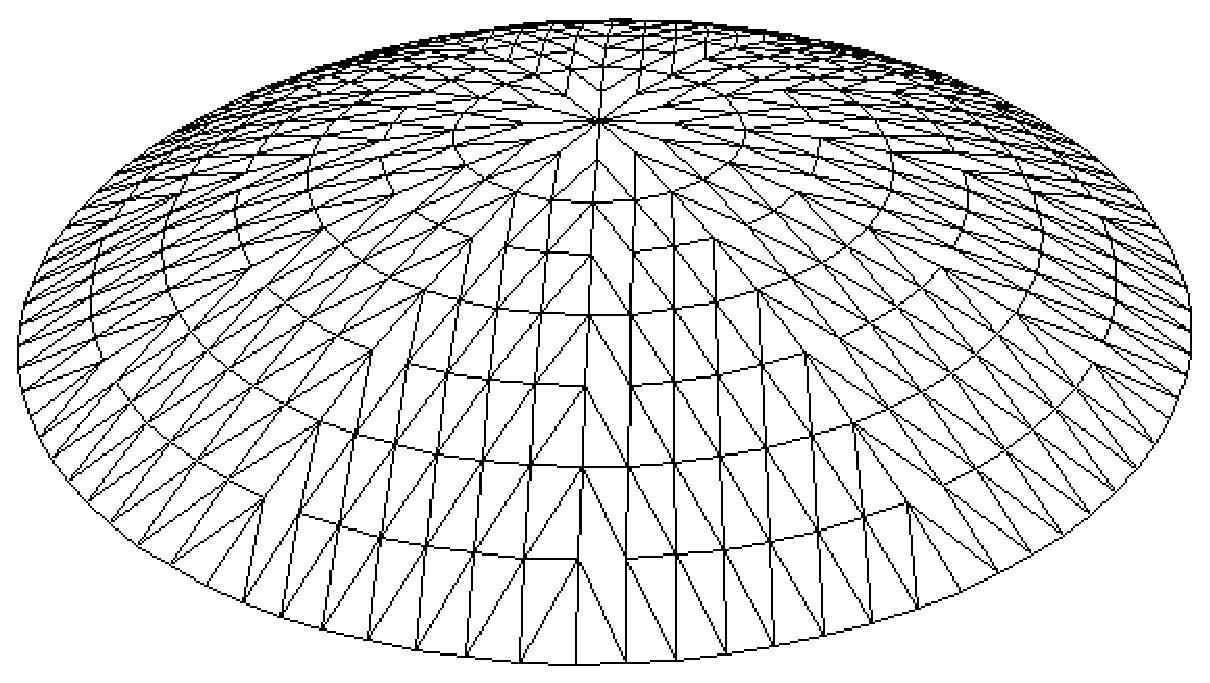
\includegraphics[height=3cm]{images/scallop}}
  \hfill
  \subfigure[Another Scallopdome]{\label{scallop2}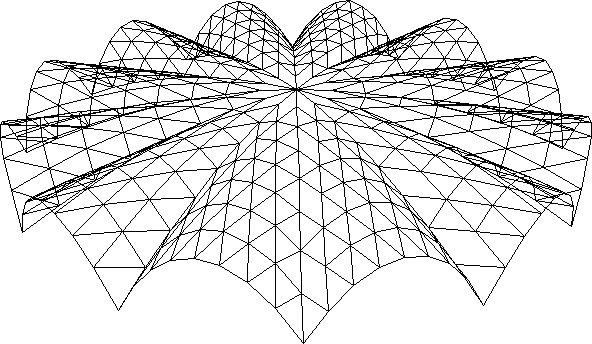
\includegraphics[height=3cm]{images/scallop2}}
  \hfill
  \subfigure[Yet another Scallopdome]{\label{scallop3}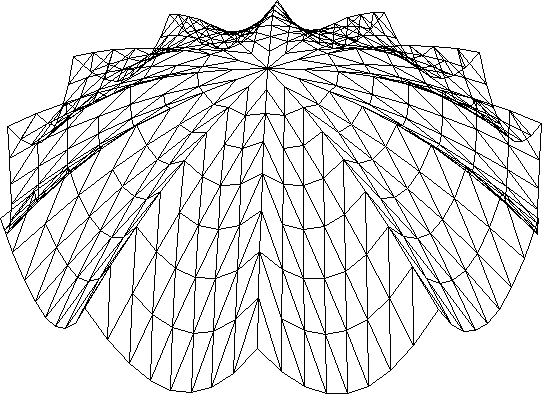
\includegraphics[height=3cm]{images/scallop3}}
  \caption{Same script, different domes}
  \label{scallops}
\end{figure}


As mentioned in the introduction, pyFormex is based on the programming language Pyhton \footnote{\url{http://www.python.org}}. This implies that the scripts are also Python-based. It's a very easy language, but if you're interested in reading more, there is a very good tutorial available on \url{http://docs.python.org/tut/}. However, if you're only using Python to write pyFormex-scripts, the tutorial you're reading right now should be enough. 

Some useful remarks when using Python and pyFormex:
\begin{itemize}
\item To open pyFormex, doubleclick on the file 'pyformex' in the installation-directory, or type 'pyformex' in the terminal. Using the terminal can be very useful, because errors that are created while running the script will appear in the terminal. This can provide you with useful information when something goes wrong with your script.
\item To make a pyFormex-script, just create a new file with your favorite text-editor and save it as 'myproject.py'.
\item To play a script, 
	\begin{itemize}
	\item select 'play' from the 'file'-menu
	\item type 'pyformex myproject.py' in the terminal. This will open pyformex and play your script at the same time
	\end{itemize}
\item In general, an argument list must have any positional arguments followed by any keyword arguments, where the keywords must be chosen from the formal parameter names. It's not important whether a formal parameter has a default value or not. No argument may receive a value more than once -- formal parameter names corresponding to positional arguments cannot be used as keywords in the same calls. %moeilijk te volgen op dit moment van de tutorial
\item identation!!

\end{itemize}

\section{Geometric model}

  
\subsection{Creating a Formex}

\subsubsection{What is a Formex}

%"technische uitleg" in andere stijl?
A Formex is a numarray of order 3 (axes 0,1,2) and type Float.
A scalar element represents a coordinate (F:uniple).

    A row along the axis 2 is a set of coordinates and represents a point
    (node, vertex, F: signet).
    For simplicity's sake, the current implementation only deals with points
    in a 3-dimensional space. This means that the length of axis 2 is always 3.
    The user can create formices (plural of Formex) in a 2-D space, but
    internally these will be stored with 3 coordinates, by adding a third
    value 0. All operations work with 3-D coordinate sets. However, a method
    exists to extract only a limited set of coordinates from the results,
    permitting to return to a 2-D environment.

    A plane along the axes 2 and 1 is a set of points (F: cantle). This can be
    thought of as a geometrical shape (2 points form a line segment, 3 points
    make a triangle, ...) or as an element in FE terms. But it really is up to
    the user as to how this set of points is to be interpreted.

    Finally, the whole Formex represents a set of such elements.

    Additionally, a Formex may have a property set, which is an 1-D array of
    integers. The length of the array is equal to the length of axis 0 of the
    Formex data (i.e. the number of elements in the Formex). Thus, a single
    integer value may be attributed to each element. It is up to the user to
    define the use of this integer (e.g. it could be an index in a table of
    element property records).
    If a property set is defined, it will be copied together with the Formex
    data whenever copies of the Formex (or parts thereof) are made.
    Properties can be specified at creation time, and they can be set,
    modified or deleted at any time. Of course, the properties that are
    copied in an operation are those that exist at the time of performing
    the operation.   

Simply put: a Formex is a set of elements, and every element can have a propertynumber.


\subsubsection{Creating a Formex Using coordinates}

The first and most useful way to create a Formex is by specifying it's nodes and elements in a 3D-list.  

\begin{verbatim}
	F=Formex([[[0,0],[1,0],[1,1],[0,1]]])
\end{verbatim}
%fig?

This would create a Formex F, which has the nodes (0,0), (0,1), (1,1) and (0,1). These nodes are all part of a single element, thus creating a square plane. This element is also the entire Formex.
On the other hand, if you would change the position of the [] %how do you call this?? square brackets?
like in the following example, then you'd create a Formex F which is different from the previous. The nodes are the same, but the connection is different. The nodes (0,0) and (1,0) are linked together by an element, and so are the nodes (1,1) and (0,1). The formex is now a set of 2 parallel bars, instead of a square plane. 
\begin{verbatim}
	F=Formex([[[0,0],[1,0]],[[1,1],[0,1]]])
\end{verbatim}
%fig?

If we want to define a Formex, simular to the square plane, but consisting of the 4 edges instead of the actual plane, we have to define four elements and combine them in a Formex.
\begin{verbatim}
F=Formex([[[0,0],[0,1]], [[0,1],[1,1]], [[1,1],[1,0]], [[1,0],[0,0]]])
\end{verbatim}

The previous examples were limited to a 2-D environment for simplicity. Of course, we could add a third dimension. For instance, it's no problem defining a pyramid consisting of 8 elements ('bars').
\begin{verbatim}
	F=Formex([[[0,0,0],[0,1,0]], [[0,1,0],[1,1,0]], [[1,1,0],[1,0,0]], [[1,0,0],[0,0,0]], [[0,0,0],[0,1,0]], [[0,0,0],[0.5,0.5,1]], [[1,0,0],[0.5,0.5,1]], [[1,1,0],[0.5,0.5,1]], [[0,1,0],[0.5,0.5,1]]])
\end{verbatim}
%fig
However, as you can see, even in this very simple example the number of nodes, elements and coordinates you have to declare becomes rather large. Defining large Formices using this method would not be practicle. This problem is easily overcome by copying, translating, rotating,... a smaller Formex - as will be explained in the rest of this chapter - or by using patterns.
 
\subsubsection{Creating a Formex Using patterns}

The second way of creating a new Formex, is by defining patterns. In this case, a line segment pattern is created from a string.

    This function creates a list of line segments where all nodes lie on the
    gridpoints of a regular grid with unit step.
    The first point of the list is [0,0]. Each character from the given
    string is interpreted as a code specifying how to move to the next node.
    Currently defined are the following codes:
    0 = goto origin [0,0]
    1 = East, 2 = North, 3 = West, 4 = South, 5 = NE, 6 = NW, 7 = SW, 8 = SE
    / = go to the next point without connecting.
    The resulting list is directly suited to initialize a Formex in the
    (x,y)-plane.

This method has important restrictions, since it can only created lines, in a 2-D environment, on a regular grid. However, it can be a much easier and shorter way to define a simple Formex. This is illustrated by the difference in lenght between code 3 and code ref 4, however they define the same Formex.
\begin{verbatim}
	F=Formex(pattern('1234'))
\end{verbatim}

\subsubsection{drawing a Formex}

Of course, you'd want to see what you have created. This is accomplished by the 'draw'-function. In code ... the pyramid we created in code ... is drawn.
\begin{verbatim}
	F=Formex([[[0,0,0],[0,1,0]], [[0,1,0],[1,1,0]], [[1,1,0],[1,0,0]], [[1,0,0],[0,0,0]], [[0,0,0],[0,1,0]], [[0,0,0],[0.5,0.5,1]], [[1,0,0],[0.5,0.5,1]], [[1,1,0],[0.5,0.5,1]], [[0,1,0],[0.5,0.5,1]]])
draw(F)
\end{verbatim}
 
It might be important to realize that even if you don't draw a particular Formex, that doesn't mean you didn't create it!

Now, when you are creating a large geometry, you might be interested in seeing the different steps in the creation. This can be accomplished by using the functions 'clear' and 'sleep'...........

\subsection{Information about a Formex}

\subsection{Changing the Formex}\label{changing F}

\subsection{Create copies, concatenations,subtractions}\label{copy F}

\subsection{Affine transformations}

\subsection{Non-affine transformations}

\subsection{Transformations that change the topology}


\section{Adding properties}

\section{Export to finite-elements program}

\section{Tips and Tricks}

Some of these tips are already mentioned in the previous sections, but......
\begin{itemize}
\item Starting pyFormex using the terminal can be very useful. Errors that are created while running the script will appear in the terminal, you can use the 'print'-function to check a result,... This can be a very useful when controlling your script
\item nog wat hints 
\end{itemize}





%%%%%%%%%%%%%%%%%%%%%%%%%%%%%%%%%%%%%%%%%%%%%%%%%%%%%%%%%%%%%%%%%%%%%%%%%%%
\chapter{pyFormex --- reference manual}
{\label{cha:reference}

\section{formex --- the base module}
{\label{sec:formex}

This module contains all the basic functionality for creating, structuring and transforming sets of coordinates.

\begin{classdesc}  {Formex}{data=[[[]]],prop=None}
A class to hold a structured set of coordinates. A \class{Formex} is a threedimensional array of float values. The array has a shape \code{(nelems,nnodel,3)}. Each slice \code{[i,j]} of the array contains the three coordinates of a point in space. We will also call this a \emph{node}. Each slice \code{[i]} of the array contains a connected set of nnodel points: we will refer to it as an \emph{element}. 

It is up to the user on how to interprete this connection: two connected nodes will usually represent a line segment between these two points. An element with three nodes however could just as well be interpreted as a triangle or as a (possibly curved) line. And if it is a triangle, it could be either the circumference of the triangle or the part of the plane inside that circumference. As far as the Formex class concerns, each element is just a set of points. 

All elements in a \class{Formex} must have the same number of points, but you can construct \class{Formex} instances with any (positive) number of nodes per element. When \code{nnodel==1}, the \class{Formex} contains only unconnected nodes (each element is just one point).

One way of attaching other data to the \class{Formex}, is by the use of the 'property' attribute. The property is an array holding one integer value for each of the elements of the Formex. The use of this property value is completely defined by the user. It could be a code for the type of element, or for the color to draw this element with. Most often it will be used as an index into some other (possibly complex) data structure holding all the characteristics of that element. 

By including this property index into the Formex class, we make sure that when new elements are constructed from existing ones, the element properties are automatically propagated.

\end{classdesc}

\begin{memberdesc}  [array]{f}
A threedimensional array of float values. The array has a shape (nelems,nnodel,3). Each slice [i,j] of the array contains the three coordinates of a point in space. We will also call this a \emph{node}. Each slice [i] of the array contains a connected set of nnodel points: we will refer to it as an \emph{element}. It is up to the user on how to interprete this connection: two connected nodes will usually represent a line segment between these two points. An element with three nodes however could just as well be interpreted as a triangle or as a (possibly curved) line. And if it is a triangle, it could be either the circumference of the triangle or the part of the plane inside that circumference.   
\end{memberdesc}



\end{document}
